\documentclass[12pt,letter]{article}
\usepackage{geometry}\geometry{top=0.75in}
\usepackage{amsmath}
\usepackage{amssymb}
\usepackage{mathtools}
\usepackage{xcolor}	% Color words
\usepackage{cancel}	% Crossing parts of equations out
\usepackage{tikz}    	% Drawing 
\usepackage{pgfplots}   % Other plotting
\usepgfplotslibrary{colormaps,fillbetween}
\usepackage{placeins}   % Float barrier
\usepackage{hyperref}   % Links
\usepackage{tikz-qtree} % Trees

%\tikzset{
%    treenode/.style = {shape=rectangle, rounded corners, draw, align=center}
%    root/.style     = {treenode, font=\Large}
%    env/.style      = {treenode, font=\ttyfamily\normalsize},
%    dummy/.style    = {circle,draw}
%}

%\tikzset{every tree node/.style={circle,align=center, anchor=west, grow=right}
%	}
\tikzset{every tree node/.style={minimum width=1em, draw, circle},
	 grow=right,
	 level distance=1.75cm}

% Don't indent
\setlength{\parindent}{0pt}
% Function to replace \section with a problem name specifically formatted
\newcommand{\problem}[1]{\vspace{3mm}\Large\textbf{{Problem {#1}\vspace{3mm}}}\normalsize\\}
% Formatting function, like \problem
\newcommand{\ppart}[1]{\vspace{2mm}\large\textbf{\\Part {#1})\vspace{2mm}}\normalsize\\}
% Formatting 
\newcommand{\condition}[1]{\vspace{1mm}\textbf{{#1}:}\normalsize\\}

\begin{document}
\title{CIS 572 Assignment 1}
\author{Steven Walton}
\maketitle
\problem{1}
Answer Exercise 3.1 from 
\href{https://www.cs.princeton.edu/courses/archive/spr07/cos424/papers/mitchell-dectrees.pdf}{Chapter 3 of Mitchell's machine learning book.}

\ppart{a} 
$$ A \wedge\neg B$$
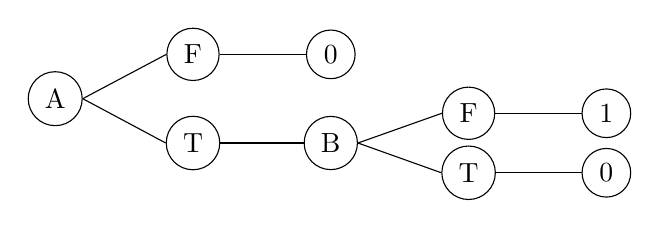
\begin{tikzpicture}
%\Tree [.A [.T [.B [.T 0 ] [.F 1 ] ] ] [.F 0 ] ]
\Tree [.A [.T [.B [.T 0 ] [.F 1 ] ] ] [.F 0 ] ]
\end{tikzpicture}


\ppart{b}
$$A\vee (B\wedge C)$$
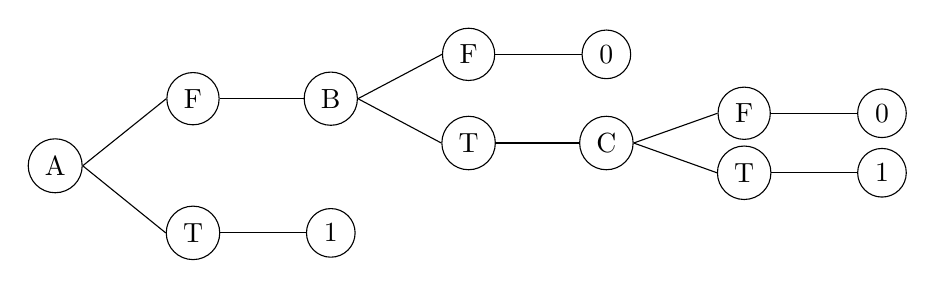
\begin{tikzpicture}
\Tree [.A [.T 1 ] [.F [.B [.T [.C [.T 1 ] [.F 0 ] ] ] [.F 0 ] ] ] ]

\end{tikzpicture}


\ppart{c}
$$ A\ \mathsf{XOR}\ B $$
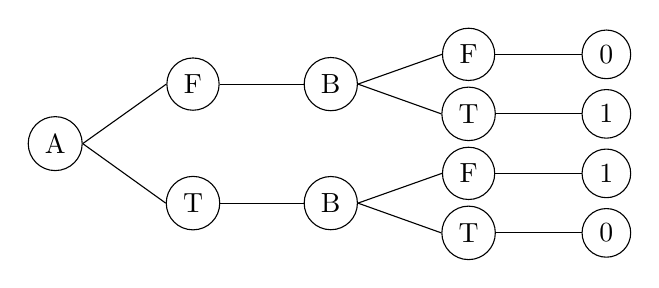
\begin{tikzpicture}
\Tree [.A [.T [.B [.T 0 ] [.F 1 ] ] ] [.F [.B [.T 1 ] [.F 0 ] ] ] ]
\end{tikzpicture}

\ppart{d}
$$ (A\wedge B)\vee(C\wedge D)$$
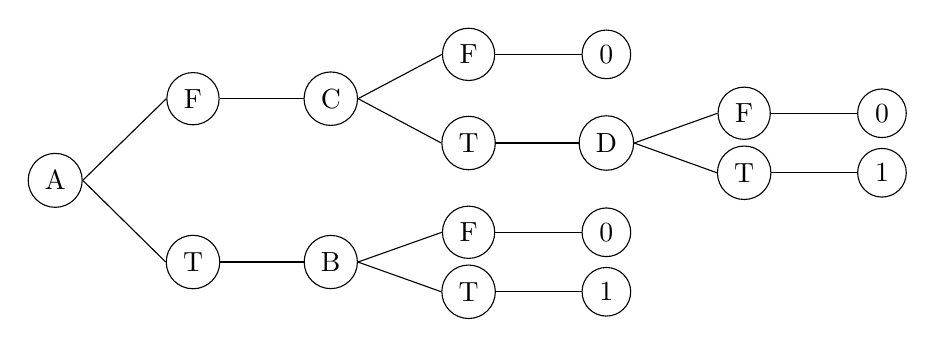
\begin{tikzpicture}
\Tree [.A [.T [.B [.T 1 ] [.F 0 ] ] ] [.F [.C [.T [.D [.T 1 ] [.F 0 ] ] ] [.F 0 ] ] ] ]
\end{tikzpicture}

\problem{2}
Consider the samples in the Play-tennis dataset from Table $3.2$ in Mitchell's
textbook. If you calculate the information-gain for all of the attributes of this
set, you will observe that the attribute ``Outlook" has the largest information-
gain, which is equal to $0.246$. Therefore, the attribute ``Outlook" is the 
best heuristic choice for the root node.
\\
(a) List the labels of the new tree branches below the root node.
\\
(b) Which partition of the data will be assigned to each branch by ID3? Please
list the sample IDs that will be assigned to each branch.
\\
(c) Calculate the information gain for the remaining attributes in each branch, 
and determine which attribute will be chosen as the root of the sub-tree in
each branch.

\ppart{a}

\ppart{b}

\ppart{c}



\end{document}
